% Save as: FamilyName_GivenName_OsloMetUsername_ACIT5900.pdf
% Compiler: XeLaTeX or LuaLaTeX

\documentclass[a4paper, 12pt, openany, british]{memoir}    % A4, 12pt, openany to not get blank pages to make chapters begin on odd pages, british/american/english
\usepackage{import}
\usepackage{preamble}   % add e.g. \usepackage{package-name} in the preamble file to avoid clutter here

%% Updates the titlepage:
\title{Title of master thesis}    % thesis title
\author{Author Name}    % Author name
\date{May 2024} % Year (update as needed)
\specialisation{Robotics and Control}   % the specialisation, e.g. Applied Artificial Intelligence
\course{ACIT5900}      % Change to ACIT5930 if long thesis


% \includeonly{} may be removed
\includeonly{
    Chapters/00abstract,
    Chapters/00preface,
    Chapters/01intro,
    Chapters/02litreview,
    Chapters/03chapter,
    Chapters/04chapter,
    Chapters/90results,
    Chapters/91discussion,
    Chapters/92conclusion,
    Chapters/appA,
    %Chapters/appB, % notice that if commented out, it will not be included even though it is included below!
}


\begin{document}

\frontmatter    % Roman numerals
\begin{titlingpage}
    \begin{center}
        %%%% Arial Bold %%%%%
        \newfontfamily{\arial}{arial-bold.ttf}[]

        \vspace*{-2mm} 
        
        \sizetf{{\arial \thecourse}} \\       % size 24pt
        \sizete{{\arial MASTER THESIS} \\}  % size 28pt
        \vspace{5mm}
        \sizett{{\arial in} \\}             % size 22pt
        \vspace{4mm}
        % 1.5 spacing, no line spacing begin
        \sizett{
        {\arial Applied Computer and Information \\
        Technology (ACIT)} \\}       % size 22pt
        %%%% Calibri %%%%%
        \vspace{2mm}
        \sizetw{\textbf{\thedate}}
        
        % Calibri 20 pt linebreak
        \vspace{11mm}    
        \sizetw{\textbf{\thespec}} \\   % Calibri bold 20pt
        \vspace{14mm}    
        \sizett{\textbf{\thetitle}}

        \vspace{28mm}
        \sizest{\theauthor} \\  % size 16pt
        \vspace{33mm}

        \sizeft{\textbf{
        Department of Computer Science \\
        Faculty of Technology, Art and Design} \\}
        \vspace{3mm}

        \begin{figure}[H]
            \centering
            \includegraphics[width=50mm, alt={Oslo Metropolitan University's logo.}]{figures/oslomet_logo.png}
            \label{fig:none}
        \end{figure}
        
        
        
        
    \end{center}
\end{titlingpage}


\RaggedRight


\chapter{\texorpdfstring{\centering Abstract}{Abstract}}
%\chapter{Abstract} % this is sufficient if 'Abstract' does not need to be centred.

\enquote{Summarise the essence of your thesis:
\begin{itemize}
    \item What was the purpose and research question/s?
    \item What was the scope of the project and how was it limited?
    \item What did you do? (Methodology)
    \item What did you discover? (Most important results)
    \item What are your conclusions and suggestions?
\end{itemize}
It must be short; ideally one page and a maximum of two.} (\cite{handbook})
\chapter{Preface}
\label{ch:preface}

\enquote{The preface is a short personal note in which you can give the reader a brief introduction to your
choice of topic and your experiences with the work. You can also use the preface to thank
individuals and institutions who have contributed along the way.

The preface ends with place and date at the time of writing, and your name and signature.} (\cite{handbook})



% Dedication, Acknowledgements, and Preface (each optional)

\tableofcontents
\newpage    
\listoffigures
\newpage
\listoftables

\newpage
%%%% OPTIONAL: List of Abbreviations or Symbols, see https://www.overleaf.com/learn/latex/Nomenclatures %%%%
\phantomsection % to add Nomenclature/Abbreviations to table of contents
\addcontentsline{toc}{chapter}{List of Abbreviations}  % title to add to table of contents
% Create groups ----------------------------
\renewcommand\nomgroup[1]{%
  \item[\bfseries
  \ifstrequal{#1}{M}{Methods}{%
  \ifstrequal{#1}{A}{Materials}{%
  \ifstrequal{#1}{F}{Factors}{}}}%
]}
% List abbreviations, for methods [M], materials [A] and factors [F] ---
\nomenclature[A]{CI}{Cast iron}
\nomenclature[A]{DI}{Ductile iron}
\nomenclature[M]{RF}{Random forest}
\nomenclature[M]{RSF}{Random survival forest}
\nomenclature[M]{DT}{Decision tree}
\nomenclature[F]{AADT}{Annual average daily traffic}

\printnomenclature
% ------------------------------------------

\mainmatter     % Arabic numerals for numbered chapters
\chapter{Introduction}
\label{ch:intro}

This is a simple and hopefully easy to use (and alter according to different requirements) \LaTeX{} implementation according to the ACIT thesis handbook which can be found in ACIT Master class in Canvas. All of the text here is copied from the handbook except for \LaTeX{} specific notes. The handbook chapter guidelines may be commented out using \% so that you have the guidelines there while writing, but they are not visible in the compiled pdf-file. 
% Like this.

The chapter file naming is done so that they are alphabetical in order, and it is easy to remove or add more chapters before the results, discussion and conclusion.

\enquote{The introduction chapter will describe the background for your project work and clearly state the theme of the thesis, goals, hypotheses or research question(s), or the product being developed. The introduction may also include an overview for the reader, which describes the main structure of the report and clarifies any special factors.

The main goal of the background section is to clarify why the project’s research questions are relevant and which challenges they intend to address. The introduction should demonstrate the
student’s knowledge of their field of study and existing research, as well as of state of the art technologies} \citep{handbook}.





\chapter{Literature Review}
\label{ch:lit-review}

\enquote{Literature reviews present and critically analyse relevant works and the relationships between
them and place the thesis within a larger context by demonstrating how work undertaken in the
thesis seeks to fill a gap in, or extend, current knowledge.

Personal opinions and points of view should not be included in this chapter.

Correct and unambiguous references must accompany all information derived from academic
literature and other relevant sources.} (\cite{handbook})

\vspace{\baselineskip} \noindent
Referencing can be done using \texttt{\textbackslash cite\{citation-key\}},
\cite{winkler2018bdt}. Page (p.), pages (pp.) or chapter (Ch.) may be specified \texttt{\textbackslash cite[here]\{citation-key\}}, e.g. \cite[pp. 2]{winkler2018bdt}. The command \texttt{\textbackslash citetitle\{citation-key\}} can be used to cite the title, e.g. \citetitle{winkler2018bdt}.

%\part{The First Part}
\chapter{Methodology}
\label{ch:1st}

\enquote{The methodology chapter should describe how data was collected or the product was produced
in a comprehensive, systematic and sufficiently detailed manner. It is important to justify the process by which the research questions, which were derived through an analysis of the relevant literature, were answered. All the methods chosen must be fully justified, and reasons for rejecting other feasible methods explained.

The documentation of which methods were used and how they were implemented should allow
other researchers to reproduce them in other studies or verify the results.

For product development projects, the choice of design and developing process(es) must be
justified and described.} (\cite{handbook})

\vspace{\baselineskip} \noindent
Note that the literature review and methodology can be placed where ever you want after \cref{ch:intro}, as long as it is before results.
\chapter{Examples}
\label{ch:04}

Preface (optional, remove from \texttt{\textbackslash includeonly} in \texttt{main.tex} if wanted). To reference a section, e.g. the literature review you can use \texttt{\textbackslash cref\{labelName\}} to reference it as \cref{ch:lit-review}. 

\enquote{This is an \enquote{inner quote} inside an outer quote}, according to the specified language's typesetting.

\vspace{\baselineskip}
\noindent
Skipping a line and dropping the indent can be used in addition to indents by using \\ \texttt{\textbackslash vspace\{\textbackslash baselineskip\}} \texttt{\textbackslash noindent} when natural.




\section{Sections can be used}
With section text. Above sections are chapters, and above that again are parts (add those in \texttt{main.tex}).

\subsection{And subsections}

\subsubsection{And subsubsections}
The subsubsection text can start right after a subsection for example.

\paragraph{And paragraphs}
Paragraphs are on the level below subsubsections.


\subparagraph{There is also subparagraphs} In summary, see \cref{tab:levels}.
\begin{table}[H]
    %\centering     % handbook says not to center!
    \caption{Memoir document class levels.}
    \begin{tabularx}{1\textwidth}{l|X}
        \textbf{Name} & \textbf{Note} \\ \hline
        Part & Add in \texttt{main.tex} \\
        Chapter & Each chapter is located under the folder \texttt{Chapters}, remember to include them in \texttt{main.tex} (in both places)! \\
        Section & \\
        Subsection & To turn of numbering and/or remove subsections from ToC, edit the preamble (search for documentclass levels). \\
        Subsubsection & \\
        Paragraph & \\
        Subparagraph & \\
    \end{tabularx}
    \label{tab:levels}
\end{table}

\LaTeX{} tables can be very compact, so the above table can easily be altered by wrapping the following around it (and the values can be changed for more or less spacing, independently):
\begin{minted}{latex}
\setlength{\tabcolsep}{0.5em}       % for the horizontal padding
{\renewcommand{\arraystretch}{1.5}  % for the vertical padding
% Table code here!
}
\end{minted}

\setlength{\tabcolsep}{0.5em}       % for the horizontal padding
{\renewcommand{\arraystretch}{1.5}  % for the vertical padding
\begin{table}[H]
    %\centering     % handbook says not to center!
    \caption{Memoir document class levels, with more spacing.}
    \begin{tabularx}{1\textwidth}{l|X}
        \textbf{Name} & \textbf{Note} \\ \hline
        Part & Add in \texttt{main.tex} \\
        Chapter & Each chapter is located under the folder \texttt{Chapters}, remember to include them in \texttt{main.tex} (in both places)! \\
        Section & \\
        Subsection & To turn of numbering and/or remove subsections from ToC, edit the preamble (search for documentclass levels). \\
        Subsubsection & \\
        Paragraph & \\
        Subparagraph & \\
    \end{tabularx}
    \label{tab:levels-space}
\end{table}
}

Also shown above, the package \texttt{minted} can also be used to display code snippets, e.g. Python code:
\begin{minted}{python}
import numpy as np

# Generate 2x3 uniformly random numbers between -1 and 1:
random_array = np.random.uniform(low=-1.0, high=1.0, size=(2,3))
\end{minted}
Note         that everything inside the \texttt{minted} environment is space sensitive, unlike       \LaTeX{} code in         general.

\subsection{Figures}
\cref{fig:logo} is an example of how to import and scale the size of figures or images, to e.g. 52 \% of the textwidth. If not required to left justify figure captions, edit the preamble (search for \enquote{captions}). Remember to add alternative text (alt text) for accessibility – a brief description of the figure for readers with visual impairments – as required in the handbook!

\begin{minted}{latex}
\begin{figure}[H]
    %\centering     % handbook says not to center!
    \includegraphics[width=0.52\textwidth, alt={Alt text here}]{figure-file.png}
    \caption{Figure caption}
    \label{fig:figure-label}
\end{figure}   
\end{minted}

\begin{figure}[H]
    %\centering     % handbook says not to center!
    \includegraphics[width=0.52\textwidth, alt={Oslo Metropolitan University's logo, in black on white.}]{oslomet_logo.png}
    \caption{Oslo Metropolitan University's logo.}
    \label{fig:logo}
\end{figure}



\section{For titles with \texorpdfstring{e.g. \(\R^3\)  or \LaTeX{}}{LaTeX code}}

For any titles with \LaTeX{} code (e.g. math mode), use the following macro provided by the \texttt{hyperref} package to provide a text-only version of the title as well: \\
\begin{minted}{latex}
    \texorpdfstring{<latex-code>}{<bookmark-text>}
\end{minted}

\vspace{\baselineskip} \noindent
This can also be seen in the abstract title, where \LaTeX{} code was used to make it centred in the displayed version:
\begin{minted}{latex}
    \chapter{\texorpdfstring{\centering Abstract}{Abstract}}
\end{minted}

\subsection{Rigid body motions in \texorpdfstring{\(\R^3\)}{real three dimensional space}}
An example how how this might be used is this title, given by
\begin{minted}{latex}
\subsection{Rigid body motions in \texorpdfstring{\(\R^3\)}{real 3-dimensional space}}
\end{minted}


%\part{The Second Part}
%\include{Chapters/05chapter}

%\part{The Final Part}
\chapter{Results}
\label{ch:results}


\enquote{This chapter presents the data or results of the research or product development. It consists of
a logical presentation of the data. The results should be organised, classified, analysed and (if relevant) categorised. Where appropriate, diagrams and tables should be used to provide an overview of the results.

The results should be explained and interpreted (e.g., differences between various studies), and
their reliability and validity should be assessed and evaluated.

Results or product developments must be presented in a clear, objective and unbiased manner.} \citep{handbook}
\chapter{Discussion}
\label{ch:discussion}

`This chapter introduces analytical and critical thinking in relation to the results or developed
product and analysis, with reference to the theoretical arguments described in the literature
review. Ensure that you allocate sufficient time to analyse, assess and relate your findings or
product to the literature.
Consider the following:
\begin{itemize}
    \item In which ways do your results or developed product agree with previous research and
    literature and what are the major differences?
    \item What is the utility value of your results or product?
    \item Which interpretations of your results can you suggest?
    \item What are the strong and weak aspects of your research?
    \item Are the results significant?
    \item Is it possible to generalise your findings?
    \item Are there any potential criticisms of your research?´
\end{itemize} (\cite{handbook})

\chapter{Conclusion}
\label{ch:conclusion}

\enquote{This chapter provides clear and concise answers to the research question(s), or addressed to the
degree to which the initial aims of the project were achieved. In addition, recommendations can
be made based on the results or developed product and pointers for useful areas for further
research.} \citep{handbook}

%\backmatter     % Arabic numerals
\printbibliography[title=References]

% Appendices, remove or comment out if none
\appendix       % Chapters are renamed "Appendix A/B/..."
\appendixpage  % like \part*{Appendices} but appears in TOC
\chapter{Some Title}
\label{app:appA}

\enquote{Include documentation that is of relevance, but too comprehensive for the report itself, as
appendices.

Appendices should not contain information that is already included in the main text of the report, but they must include material referred to in the report.

Examples of appendices:
\begin{itemize}
    \item Additional details of methods and/or data
    \item Diagrams of specialised equipment developed
    \item Interview guides, interview questions and anonymous raw data from interviews
    \item Questionnaires or surveys used in the research
    \item Prototype(s)
    \item Development description(s)
    \item User, design and product requirements
    \item Sketches
    \item Program codes with references
    \item Tables and analyses
\end{itemize}
If relevant/necessary, appendices may be in their original format (e.g. program coding, images,
sound and video), and may then be submitted in additional file(s).
List and number the appendices at the end of the report.} (\cite{handbook})


\vspace{\baselineskip} \noindent
Note that Appendix B is not visible, because it is commented out in \texttt{\textbackslash includeonly\{\}} in \texttt{main.tex}.
\chapter{Appendix B Title}
\label{app:appB}

Note that this appendix is not visible, because it is commented out in \texttt{\textbackslash includeonly\{\}}.


\end{document}


